\section{Fractures and dual porosity}

File: \texttt{06\_frac\_dualpor.yaml}

\subsection{Description}

This is a variant of \texttt{04\_frac\_diffusion.yaml}. Instead of
diffusion we consider advective transport with dual porosity.

\subsection{Input}

Dual porosity substitutes blind fractures in this task. The
dual-porosity parameter \texttt{diffusion\_rate\_immobile} was
calibrated to the value 5.64742e-06 for identical results with the model
with the blind fractures. Other settings of transport are identical to
the diffusion model.

The dual porosity model is set by the following lines:

\begin{verbatim}
reaction_term: !DualPorosity
  input_fields:
    - region: rock
      init_conc_immobile: 0
    - region: flow_fractures
      diffusion_rate_immobile: 5.64742e-06
      porosity_immobile: 0.01
      init_conc_immobile: 0
    - region: blind_fractures
      init_conc_immobile: 0
\end{verbatim}

\subsection{Results and comparison}

Results of calibration of the model with dual porosity and model with
flow in blind fractures (file \texttt{06\_frac\_nodualpor.yaml}) is
depicted in Figure \ref{fig:calib}.

\begin{figure}[htbp]
\centering
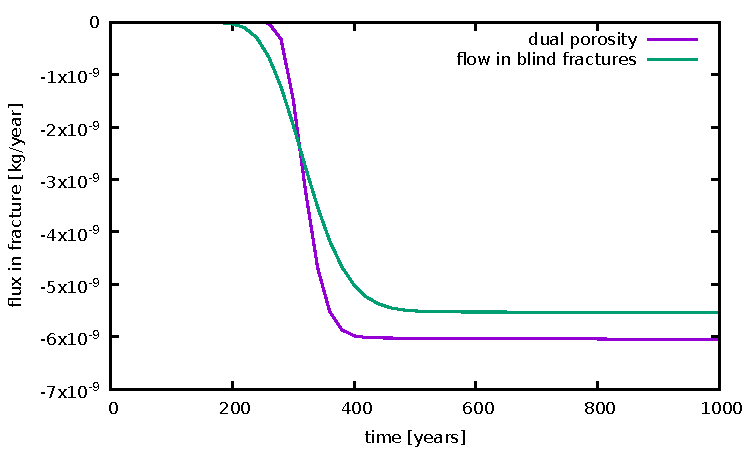
\includegraphics{tutor_figures/06_mass_flux.pdf}
\caption{Results of calibration.\label{fig:calib}}
\end{figure}
